\documentclass[12pt]{article}
\usepackage{listings}
\usepackage{graphicx}

\usepackage{xcolor}
\definecolor{codegreen}{rgb}{0,0.6,0}
\definecolor{codegray}{rgb}{0.5,0.5,0.5}
\definecolor{codepurple}{rgb}{0.58,0,0.82}
\definecolor{backcolour}{rgb}{0.95,0.95,0.92}

\lstdefinestyle{mystyle}{
    backgroundcolor=\color{backcolour},   
    commentstyle=\color{codegreen},
    keywordstyle=\color{magenta},
    numberstyle=\tiny\color{codegray},
    stringstyle=\color{codepurple},
    basicstyle=\ttfamily\footnotesize,
    breakatwhitespace=false,         
    breaklines=true,                 
    captionpos=b,                    
    keepspaces=true,                 
    numbers=left,                    
    numbersep=5pt,                  
    showspaces=false,                
    showstringspaces=false,
    showtabs=false,                  
    tabsize=2
}

\lstset{style=mystyle}

\begin{document}

\section*{Introduction}
I checked whether the site likelihoods of an inferred tree from the
language dataset, have the same distribution as the likelihoods from data
that have been indeed produced by the tree itself. I did the same for
the parsimony scores of the sites for the maximum likelihood tree. 

\section*{The Code}
\lstinputlisting[language=R]{checkphylo.R}

\section*{Results}
The main results are presented in the two figures below

\begin{figure}[htbp!]
  \centering
  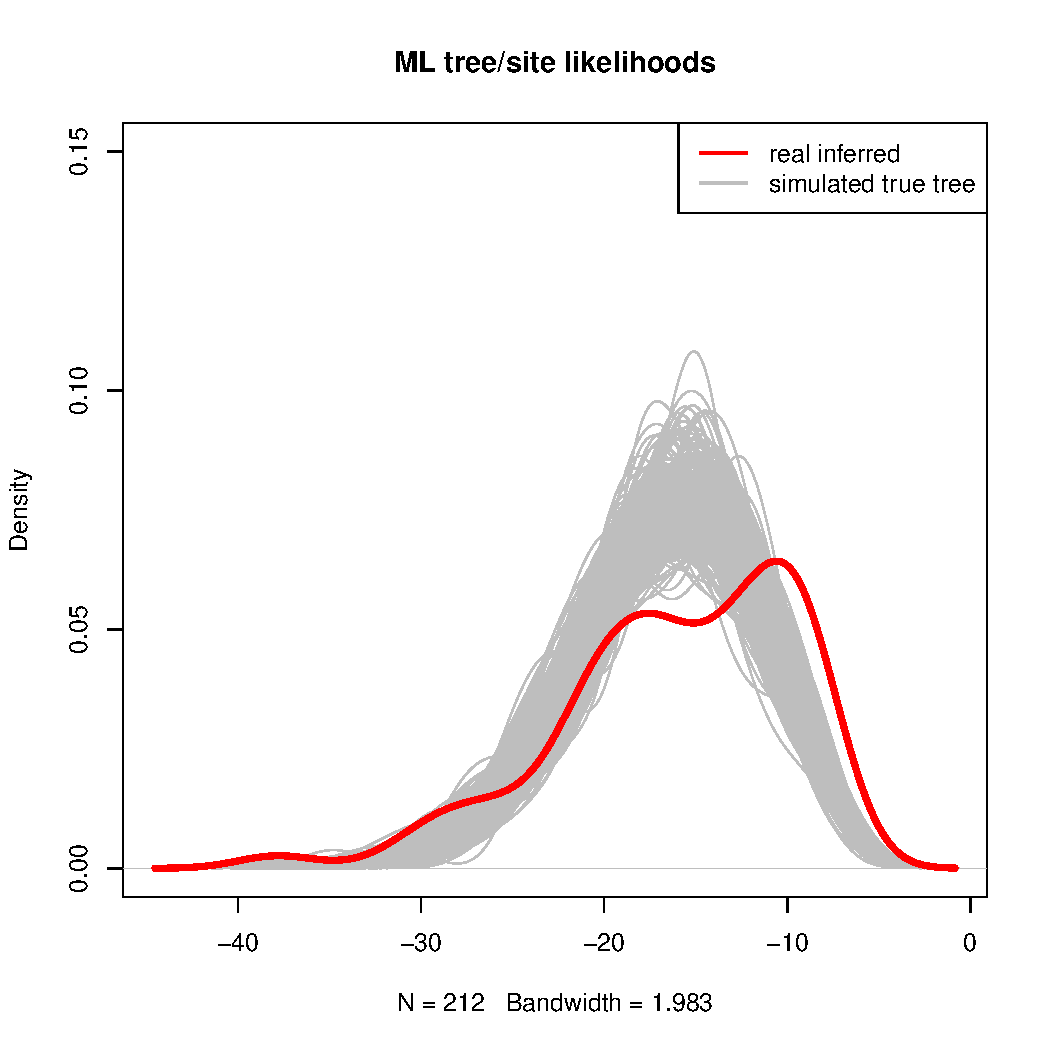
\includegraphics[width=\textwidth]{siteMLValues.pdf}
  \caption{gray color: simulated data on the same ML tree as the inferred
    tree. Red color: real data on the inferred tree. Each line
    represents the density plot of the site likelihoods. }
\end{figure}

\begin{figure}[htbp!]
  \centering
  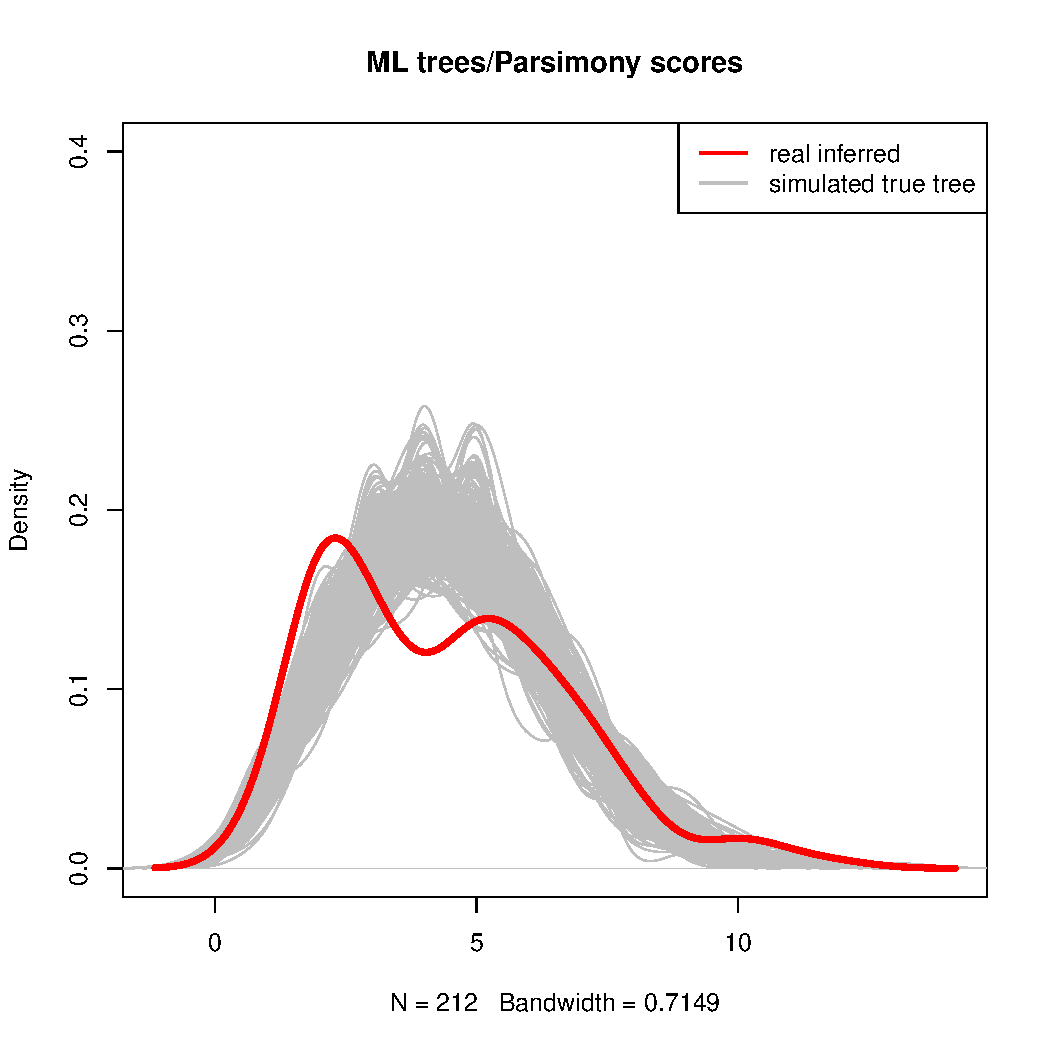
\includegraphics[width=\textwidth]{siteParsValues.pdf}
  \caption{gray color: simulated data on the same ML tree as the inferred
    tree. Red color: real data on the inferred tree. Each line
    represents the density plot of the site parsimony scores. }
\end{figure}

\section*{Conclusion}
It seems that the red distribution is qualitatively different than the
gray ones. This may mean that the tree inferred from the language
data, in fact, might be a non-correct tree. However, I understand that
this is not a right way to show this. It's interesting that the
distribution shows two peaks. Thus, it might be that in fact I have a
mixture of two distributions, i.e., some sites produce a good score
and some other a much worse score. 


\end{document}
